We shall discuss the computation of some basic operations on template
complex zonotopes like linear transformation, Minkowski sum and
intersection in special cases.  In the next section, we shall discuss
how to check inclusion between two template complex zonotopes.  For
the rest of this chapter, we use the following notation, unless
otherwise specified.
%
\begin{align*}
\ptemp\in\mat{n}{m}{\compnums},~~\sfact\in\reals^m_{\geq 0},~~\cen\in\reals^n.
\end{align*}
%
The set of template complex zonotopes is closed under linear transformation and
{Minkowski sum} operations, which are straightforward algebraic
computations just like in the case of simple (real) zonotopes.
%
\begin{lemma}[Linear transformation]~\label{lem:lin-transform}
Let $A\in\mat{n}{n}{\reals}$ and $\ptemp\in\mat{n}{m}{\compnums}$.

%
\begin{equation*}~\label{eqn:lin-transform}
\text{Then}~~~~A\tcztope{\ptemp}{\cen}{\sfact}=\tcztope{A\ptemp}{A\cen}{\sfact}.
\end{equation*}
%
\end{lemma}
%
\begin{proof}
  We derive
  %
  \begin{align*}
&
    A\tcztope{\ptemp}{\cen}{\sfact}=A\set{\cen+\ptemp\zeta:~\zeta\in\compnums^m,~\absolute{\zeta}\leq
    \sfact}\\
    & =\set{A\cen+A\ptemp\zeta:~\zeta\in\compnums^m,~\absolute{\zeta}\leq
    \sfact}=\tcztope{A\ptemp}{A\cen}{\sfact}.~\hspace{3em}\qedhere
  \end{align*}
  %
\end{proof}
%
We see that the template of a complex zonotope can change after a
linear transformation.  But when the column vectors of the template
are the eigenvectors of the linear transformation and the center is
the origin, we can represent the transformed complex zonotope using
the same template by multiplying the scaling factors with the
magnitudes of eigenvalues.  So, when the magnitudes of eigenvalues are
less than one, the transformed template complex zonotope contains the
original template complex zonotope.  This result can be seen as an
extension of Proposition~\ref{lem:eig-invariance} to the case of
template complex zonotopes.
%
\begin{lemma}[Eigenstructure based scaling]~\label{lem:eig-scaling}
Let us consider $\ptemp\in\mat{n}{n}{\compnums}$ consists of the complex
eigenvectors of a matrix $A\in\mat{n}{n}{\reals}$ as the column vectors.
Let $\mu\in\compnums^n$ be the vector of eigenvalues such that
$A\ptemp=\ptemp\diagonal{\mu}$.
%
\begin{equation}~\label{eqn:eigen-scaling}
\text{Then}~~A\tcztope{\ptemp}{0}{\sfact}=\tcztope{\ptemp}{0}{\diagonal{\absolute{\mu}}\sfact}.
\end{equation}
%
\end{lemma}
%
\begin{proof}
Based on Equation~\ref{eqn:lin-transform} and the fact that
$A\ptemp=\ptemp\diagonal{\mu}$, we get
%
\[
A\tcztope{\ptemp}{0}{\sfact}=\tcztope{A\ptemp}{0}{\sfact}=\tcztope{\ptemp\diagonal{\mu}}{0}{\sfact}.
\]
%
Then using Equation~\ref{eqn:normalization}, we get
%
\[
\tcztope{\ptemp\diagonal{\mu}}{0}{\sfact}=\tcztope{\ptemp}{0}{\diagonal{\absolute{\mu}}\sfact}.~\hspace{3em}\qedhere
\]
\end{proof}

The Minkowski sum of two template complex zonotopes is another
template complex zonotope, which is computed as follows.
%
\begin{lemma}[Minkowski sum]~\label{lem:min-sum}
Let us consider two templates ${\ptemp\in\mat{n}{m}{\compnums}}$ and
${\ptemp^\pr\in\mat{n}{r}{\compnums^r}}$.  We get
%
\begin{equation}
\minsum{\tcztope{\ptemp}{\cen}{\sfact}}{\tcztope{\ptemp^\pr}{\cen^\pr}{\sfact^\pr}}
= \tcztope{\begin{bmatrix}\ptemp & \ptemp^\pr\end{bmatrix}}{\cen+\cen^\pr}{\begin{bmatrix}\sfact\\\sfact^\pr\end{bmatrix}}
\end{equation}
\end{lemma}
%
\begin{proof}
We derive the following.
%
\begin{align*}
&
  \tcztope{\ptemp}{\cen}{\sfact}\oplus\tcztope{\ptemp^\pr}{\cen^\pr}{\sfact^\pr}\\
& =
  \set{\cen+\ptemp\zeta:~\zeta\in\compnums^m,~\absolute{\zeta}\leq\sfact}\oplus\set{\cen^\pr+\ptemp\zeta^\pr:~\zeta^\pr\in\compnums^r,~\absolute{\zeta^\pr}\leq\sfact^\pr}\\
& =
  \set{\lt(\cen+\cen^\pr\rt)+\ptemp\zeta+\ptemp^\pr\zeta^\pr:~\zeta\in\compnums^m,~\zeta^\pr\in\compnums^r,~\absolute{\zeta}\leq\sfact,~\absolute{\zeta^\pr}\leq\sfact^\pr}\\
& =
  \set{\lt(\cen+\cen^\pr\rt)+\mymatrix{\ptemp&\ptemp^\pr}\mymatrix{\zeta\\\zeta^\pr}:~\mymatrix{\zeta\\\zeta^\pr}\in\compnums^{m+r},~\absolute{\mymatrix{\zeta\\\zeta^\pr}}\leq\mymatrix{\sfact\\\sfact^\pr}}\\
& =  \tcztope{\begin{bmatrix}\ptemp & \ptemp^\pr\end{bmatrix}}{\cen+\cen^\pr}{\begin{bmatrix}\sfact\\\sfact^\pr\end{bmatrix}}.~\hspace{3em}\qedhere
\end{align*}
%
\end{proof}
%
We see that that the representation size of a template complex
zonotope can increase after a Minkowski sum with another template
complex zonotope.  But when two template complex
zonotopes have the same template, their Minkowski sum results in a
complex zonotope with the same template, i.e., the representation size
does not increase.  This is described in the following Proposition.
%
\begin{proposition}[Minkowski sum with common template]~\label{prop:commin}
The following is true.
%
\begin{equation}~\label{eqn:common-minkowski}
\minsum{\tcztope{\ptemp}{\cen}{\sfact}}{\tcztope{\ptemp}{\cen^\pr}{\sfact^\pr}}=\tcztope{\ptemp}{\cen+\cen^\pr}{\sfact+\sfact^\pr}
\end{equation}
%
\end{proposition}
%
\begin{proof}
We have $\minsum{\tcztope{\ptemp}{c}{s}}{\tcztope{\ptemp}{c^\pr}{s^\pr}}=$
%
\begin{align}~\label{eqn:proof-commin2}
&
\set{\lt(\cen+\ptemp\zeta\rt)+\lt(\cen^\pr+\ptemp\zeta^\pr\rt):\zeta,\zeta^\pr\in\compnums^m,~\absolute{\zeta}\leq
\sfact,~\absolute{\zeta^\pr}\leq \sfact^\pr}\nonumber\\
& = \set{\lt(\cen+\cen^\pr\rt)+\ptemp\lt(\zeta+\zeta^\pr\rt):\zeta,\zeta^\pr\in\compnums^m,~\absolute{\zeta}\leq
\sfact,~\absolute{\zeta^\pr}\leq \sfact^\pr}
\end{align}
%
We shall show that
\begin{equation}~\label{eqn:proof-commin1}
\set{\zeta+\zeta^\pr:\zeta,\zeta^\pr\in\compnums^m,~\absolute{\zeta}\leq
\sfact,~\absolute{\zeta^\pr}\leq\sfact^\pr}=\set{\zeta^\dpr:\absolute{\zeta^\dpr}\leq\sfact+\sfact^\pr }.
\end{equation}
%
First we shall show that the L.H.S of Equation~\ref{eqn:proof-commin1} is
contained within the R.H.S of Equation~\ref{eqn:proof-commin1}, as follows.  Let
us consider
%
\[
\zeta,\zeta^\pr\in\compnums^m:~~\absolute{\zeta}\leq
\sfact,~\absolute{\zeta^\pr}\leq\sfact^\pr.
\]
%
Then using the triangular inequality, we get
%
\begin{align*}
\absolute{\zeta_i+\zeta^\pr_i}\leq
\absolute{\zeta_i}+\absolute{\zeta^\pr_i}=\sfact+\sfact^\pr
\end{align*}
%
First we shall show that the R.H.S of Equation~\ref{eqn:proof-commin1} is
contained within the L.H.S of Equation~\ref{eqn:proof-commin1}, as follows.  
Let us consider
%
\[
\zeta^\dpr\in\compnums:~\absolute{\zeta^\dpr}\leq \sfact+\sfact^\pr.
\]
%
Let us consider
%
\[
\zeta=\sfact\frac{\zeta^\dpr}{\sfact+\sfact^\pr},~~\zeta^\pr=\sfact^\pr\frac{\zeta^\dpr}{\sfact+\sfact^\pr}.
\]
%
So, $\zeta^\dpr=\zeta+\zeta^\pr$.  As
$\absolute{\frac{\zeta^\dpr}{\sfact+\sfact^\pr}}\leq 1$, we get
$\absolute{\zeta}\leq \sfact$ and
$\absolute{\zeta^\pr}\leq\sfact^\pr$.  This proves that
the R.H.S of Equation~\ref{eqn:proof-commin1} is contained inside the
L.H.S of Equation~\ref{eqn:proof-commin1}.

Hence, we have proved Equation~\ref{eqn:proof-commin1}.  Then the
proposition follows from
Equations~\ref{eqn:proof-commin2} and~\ref{eqn:proof-commin1}.
\end{proof}
%
We denote the value of the support function of a set $\Psi\in\reals^n$
at a vector $v\in\reals^n$ as $\supp{v}{\Psi}$, which is defined as
follows.
%
\[
\supp{v}{\Psi}=\sup_{x\in\Psi}v^Tx.
\]
%
The support function of a template complex zonotope is an affine
expression of the scaling factors and the center, as described in the
following lemma.
%
\begin{lemma}[Support function]~\label{lem:support-tcz}
Let $v\in\reals^n$.  Then
%
\begin{align*}
& \supp{v}{\real\lt(\tcztope{\ptemp}{\cen}{\sfact}\rt)}=v^Tc+\absolute{v^T\ptemp}\sfact.
\end{align*}
%
\end{lemma}
%
\begin{proof}
We derive
%
\begin{align*}
&
  \supp{v}{\real\lt(\tcztope{\ptemp}{\cen}{\sfact}\rt)}=\max_{x\in\real\lt(\tcztope{\ptemp}{\cen}{\sfact}\rt)}v^Tx\\
& =
  v^T\cen+\max_{\zeta\in\compnums^m:~\absolute{\zeta}\leq\sfact}\real\lt(v^T\ptemp\zeta\rt)~\numberthis\label{proof-supp-tcz3}\\
& \leq
  v^T\cen+\max_{\zeta\in\compnums^m:~\absolute{\zeta}\leq\sfact}\absolute{v^T\ptemp}\absolute{\zeta}\\
& \leq v^T\cen+\max_{y\in\reals_{\geq 0}^m:y\leq \sfact}\absolute{v^T\ptemp}y=v^T\cen+\absolute{v^T\ptemp}\sfact.~\numberthis\label{proof-support-tcz}
\end{align*}
%
Let us consider
$\epsilon\in\compnums^m$ where
%
\[
\forall i\in\set{1,...,m},~\epsilon_i=\frac{\absolute{v^T\ptemp}_i}{\lt(v^T\ptemp\rt)_i}\sfact_i.
\]
%
Then we derive the following.
%
\begin{align*}
& \forall
  i\in\set{1,...,m},~\absolute{\epsilon_i}=\frac{\absolute{v^T\ptemp}_i}{\absolute{v^T\ptemp}_i}\absolute{\sfact_i}=\sfact_i.~\numberthis\label{proof-supp-tcz1}\\
&
  v^T\epsilon=\sum_{i=1}^m\lt(v^T\ptemp\rt)_i\frac{\absolute{v^T\ptemp}_i}{\lt(v^T\ptemp\rt)_i}\sfact_i\\
& = \absolute{v^T\ptemp}\sfact.~\numberthis\label{proof-supp-tcz2}
\end{align*}
%
By Equations~\ref{proof-supp-tcz3},~\ref{proof-supp-tcz1},
and~\ref{proof-supp-tcz2}, we get
%
\begin{equation}
\supp{v}{\real\lt(\tcztope{\ptemp}{\cen}{\sfact}\rt)}\geq v^T\cen+\absolute{v^T\ptemp}\sfact~\label{proof-supp-tcz4}
\end{equation}
%
The Lemma follows from Equations~\ref{proof-support-tcz} and~\ref{proof-supp-tcz4}.
\end{proof}
%
Like real zonotopes, complex zonotopes are also not closed under
mutual intersection.  Even the intersection between template complex
zonotopes with a common template and center need not be a closed.  But
when the common template is a non-singular (invertible) matrix and
the center is common, then the intersection is a closed operation and
can be expressed algebraically.
%
\begin{example}
Let us consider two template complex zonotopes having a common
template as $\tcztope{\ptemp}{0}{\sfact}$ and
$\tcztope{\ptemp}{0}{\sfact^\pr}$ where
%
\[
V = \mymatrix{
  1+\iota & 1 & 0\\
  1 & 0 & 1
},~~
\sfact=\mymatrix{1\\0.5\\1}~\text{and}~\sfact^\pr=\mymatrix{1\\1\\0.5}.
\]
%
The template complex zonotope
$\tcztope{V}{0}{\meet{\sfact}{\sfact^\pr}}$, where
$\meet{\sfact}{\sfact^\pr}=\mymatrix{1 & 0.5 & 0.5}^T$, can not be an
over-approximation of the intersection of the previous two template
complex zonotopes as shown in Figure~\ref{fig:nonclosure}.

On the other hand, let us consider the following invertible matrix $W$
and two vectors of scaling factors $r$ and $r^\pr$, respectively.
%
\[
W=\mymatrix{0.5+\iota & 0\\ 0.5 & 1},~~r=\mymatrix{1\\0.5},~~r^\pr=\mymatrix{0.5\\1}.
\]
%
Since $W$ is invertible, we can exactly express the intersection
between the two complex zonotopes as another complex zonotope given
below and illustrated in Figure~\ref{fig:closure}.
%
\[
\tcztope{W}{0}{r}\bigcap\tcztope{W}{0}{r^\pr} = \tcztope{W}{0}{\meet{r}{r^\pr}}.
\]
%
\end{example}
%
\begin{figure}
  \center
  \caption{Non-closure of intersection between complex zonotopes for a non-invertible template.}~\label{fig:nonclosure}
  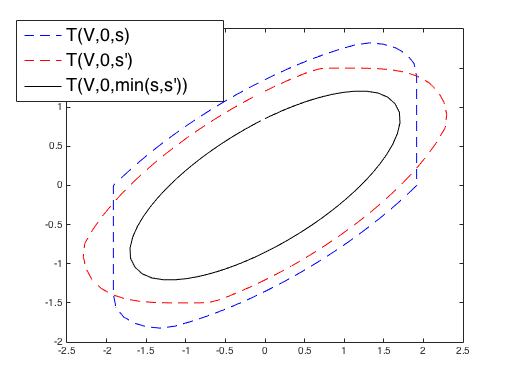
\includegraphics[scale=0.5]{fig/CZtopes/nonclosure.png}
  \vspace{1em}
  \caption{Closure of intersection between complex zonotopes for an invertible template.}~\label{fig:closure}
  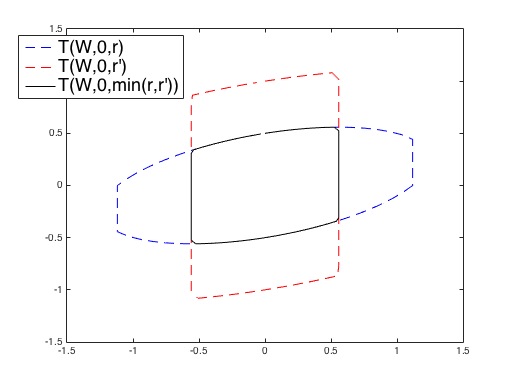
\includegraphics[scale=0.5]{fig/CZtopes/closure.png}
\end{figure}
%

The observation in the above example about intersection between
complex zonotopes is mathematically explained for a general case in
the following lemma.
%
\begin{lemma}[Mutual intersection]~\label{lem:intersection}
Let ${\ptemp\in\mat{n}{n}{\compnums}}$ be a non-singular matrix.  

%
\begin{equation}~\label{eqn:intersection}
\text{Then}\hspace{1em}\tcztope{\ptemp}{\cen}{\sfact}\bigcap\tcztope{\ptemp}{\cen}{\sfact^\pr}=\tcztope{\ptemp}{\cen}{\meet{\sfact}{\sfact^\pr}}.
\end{equation}
%
\end{lemma}
%
\begin{proof}
  Let us consider a
point $z\in\tcztope{\ptemp}{\cen}{\meet{\sfact}{\sfact^\pr}}$ where
%
\begin{align*}
& z=c+\ptemp\zeta:~\absolute{\zeta}\leq \meet{\sfact}{\sfact^\pr}.
 \text{Then}\hspace{1em}\absolute{\zeta}\leq\sfact,\hspace{1em}
  \absolute{\zeta}\leq \sfact^\pr\\
& \implies {z\in\tcztope{\ptemp}{\cen}{\sfact}}~\wedge~
           {z\in\tcztope{\ptemp}{\cen}{\sfact^\pr}}
 \implies z\in
\tcztope{\ptemp}{\cen}{\sfact}\bigcap\tcztope{\ptemp}{\cen}{\sfact^\pr}.           
\end{align*}
%
This proves that the L.H.S of Equation~\ref{eqn:intersection}
is contained inside the R.H.S.

Now let us consider a point
$x\in\tcztope{\ptemp}{\cen}{\sfact}\bigcap\tcztope{\ptemp}{\cen}{\sfact^\pr}$.
Let us express $x$ as 
%
\[
x=\cen+\ptemp\zeta.
\]
%
Since $\ptemp$ is an invertible matrix, we have a unique solution for
$\zeta$, i.e.,
$\zeta=\ptemp^{-1}\lt(x-\cen\rt)$.  As
${x\in\tcztope{\ptemp}{\cen}{\sfact}}
\bigcap\tcztope{\ptemp}{\cen}{\sfact^\pr}$ and $\zeta$ has unique solution, we get
%
\begin{align*}
  &  \absolute{\zeta}
 \leq
\sfact~\wedge~\absolute{\zeta}\leq
\sfact^\pr.\\
& \implies \absolute{\zeta}\leq\meet{\sfact}{\sfact^\pr}
\implies x\in\tcztope{\ptemp}{\cen}{\meet{\sfact}{\sfact^\pr}}.
\end{align*}
%
The above means that the R.H.S of Equation~\ref{eqn:intersection} is
contained inside the L.H.S.  The converse was proved earlier.  So, we
have proved the Lemma.
\end{proof}
%
Since template complex zonotopes are not closed under intersection,
generally there is no smallest over-approximation of a given set by a
template complex zonotope.  But according to
Lemma~\ref{lem:intersection}, template complex zonotopes with a fixed
invertible template matrix and fixed center are closed under mutual
intersection.  Therefore, for a fixed invertible template and fixed center, there
exists a smallest template complex zonotope approximation of a given
set, expressed as follows.
%
\begin{theorem}~\label{thm:min-abstraction}
Let $\Psi\subseteq\compnums^n$ be a bounded set and
$\ptemp\in\mat{n}{n}{\compnums}$ be an invertible square matrix.
Let us consider %
\[
S=\set{\sfact\in\reals_{\geq
    0}^n:\Psi\subseteq\tcztope{\ptemp}{\cen}{\sfact}}
\]
Then all of the following is true.
%
\begin{align*}
& \Psi\subseteq\bigcap_{\sfact\in
    S}\tcztope{\ptemp}{\cen}{\sfact}=\tcztope{\ptemp}{\cen}{\vectormin{s\in
  S}s}.~\numberthis\label{eqn:min-abstraction1}\\
& \vectormin{s\in S}s=\vectormax{x\in \Psi}\absolute{\inv{\ptemp}\lt(x-\cen\rt)}.~\numberthis\label{eqn:min-abstraction2}
\end{align*}
%
\end{theorem}
%
\begin{proof}
  First, we shall prove Equation~\ref{eqn:min-abstraction1}.
Based on Lemma~\ref{lem:intersection}, it follows that
%
\[
\bigcap_{\sfact\in
S}\tcztope{\ptemp}{\cen}{\sfact}=\tcztope{\ptemp}{\cen}{\vectormin{s\in
S}s}.
\]
%
As $S$ is the set of all scaling factors
whose corresponding template complex zonotope is an over-approximation
of $\Psi$, we also get
%
\[
\Psi\subseteq\bigcap_{\sfact\in
  S}\tcztope{\ptemp}{\cen}{\sfact}=\tcztope{\ptemp}{\cen}{\vectormin{s\in
  S}s}.
\]
%
So, we have proved Equation~\ref{eqn:min-abstraction1}.

Now we shall prove Equation~\ref{eqn:min-abstraction2}.  We shall
first prove
%
\begin{equation}
  \Psi\subseteq\tcztope{\ptemp}{\cen}{\vectormax{x\in \Psi}\absolute{\inv{\ptemp}\lt(x-\cen\rt)}}.~\label{proof-abstraction1}
\end{equation}
%
Let us
consider a point $x\in\Psi$.  Since $\ptemp$ is invertible, $x$ can be
written as a linear combination of template column vectors
of $\ptemp$ plus the center $\cen$ as
\[x=\cen+\ptemp\lt(\inv{\ptemp}\lt(x-\cen\rt)\rt),\] where the vector of
combining coefficients is $\lt(\inv{\ptemp}\lt(x-\cen\rt)\rt)$.  Since
%
\begin{align*}
& \absolute{\inv{\ptemp}\lt(x-\cen\rt)}\leq\vectormax{x\in \Psi}\absolute{\inv{\ptemp}\lt(x-\cen\rt)},\\
  & \text{we get},\hspace{1em} x\in\tcztope{\ptemp}{\cen}{\vectormax{x\in \Psi}\absolute{\inv{\ptemp}\lt(x-\cen\rt)}}.
\end{align*}
%
As the above is true for any $x\in\Psi$, we have proved
Equation~\ref{proof-abstraction1}.  By
Equation~\ref{proof-abstraction1} and the definition of $S$,
we get $\vectormax{x\in
  \Psi}\absolute{\inv{\ptemp}\lt(x-\cen\rt)}\in S$.  Therefore,
%
\begin{align*}
\vectormin{s\in S}s\leq\vectormax{x\in\Psi}\absolute{\inv{\ptemp}\lt(x-\cen\rt)}.~\numberthis\label{proof-abstraction2}
\end{align*}
%
By Equation~\ref{eqn:min-abstraction1}, which we have proved earlier, and
the fact that $x\in\Psi$, we
get
%
\begin{align*}
& x\in\tcztope{\ptemp}{\cen}{\vectormin{s\in
      S}s}.
\end{align*}
%
Since $\inv{\ptemp}\lt(x-\cen\rt)$ is the unique vector of combining
coefficients when $x$ is expressed as a linear combination of column
vector of $\ptemp$, the above implies
%
\begin{align*}
& \absolute{\inv{\ptemp}\lt(x-\cen\rt)}\leq\vectormin{s\in S}s.
\end{align*}
%
As the above equation is true for any $x$ in $\Psi$, we get
%
\begin{align*}
\vectormax{x\in\Psi}\absolute{\inv{\ptemp}\lt(x-\cen\rt)}\leq\vectormin{s\in\Psi}s.
\end{align*}
%
Based on the above equation and Equation~\ref{proof-abstraction2},
we get Equation~\ref{eqn:min-abstraction2}.
\end{proof}

